\section{Architecture}

\subsection{Implementation}

We developed the architecture later illustrated keeping in mind that we have a single immutable database on which we write (historical database) and possible multiple databases or data sources from which to read.

To interface on these databases or data sources we thought to use multiple adapters to transform the data coming in a writable format on hisotircal database.

\subsection{Adapter Pattern}

\begin{center}
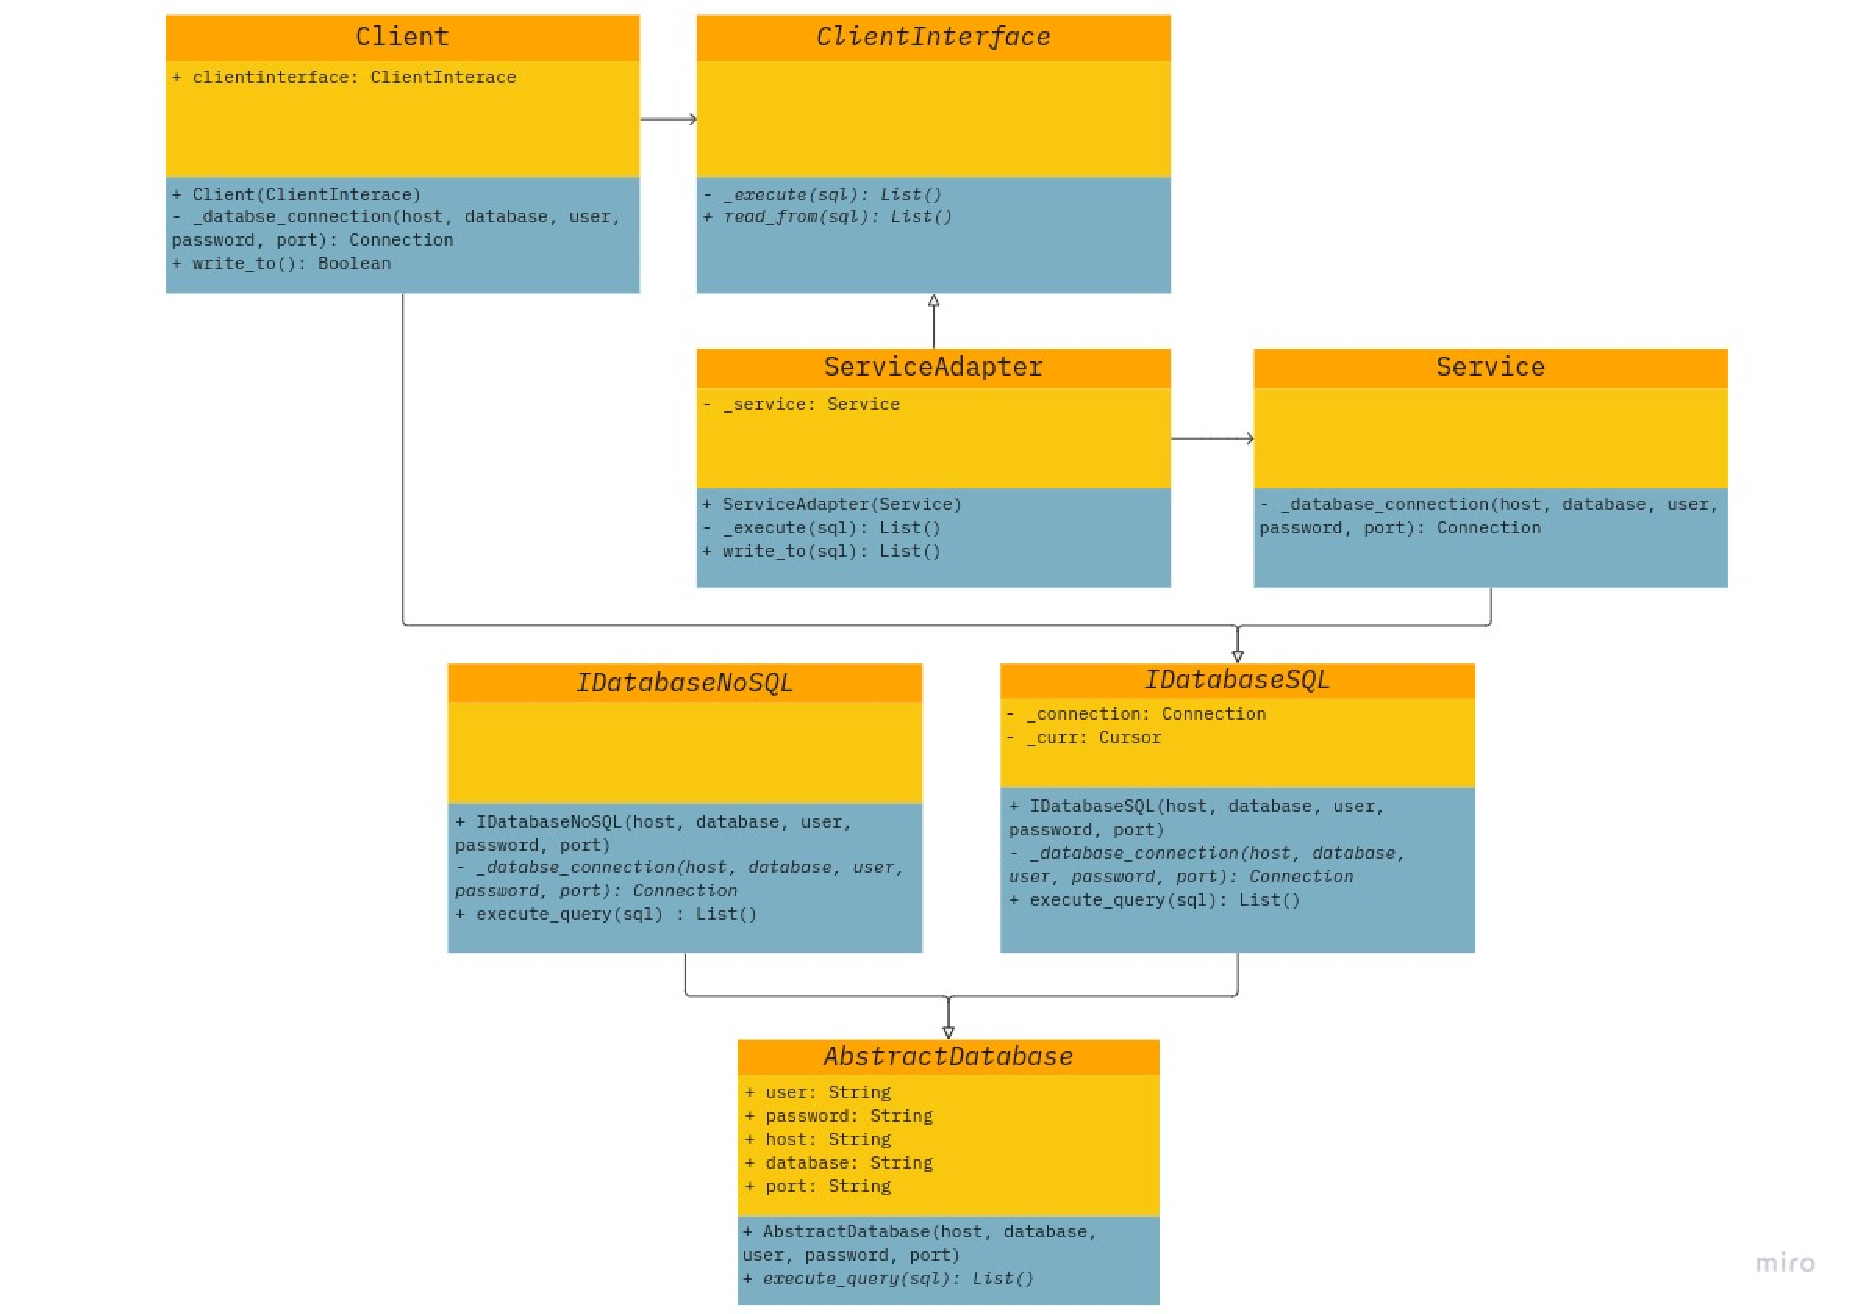
\includegraphics[scale=0.45]{uml-diagram}
\end{center}

\textbf{Please note: The gray part is not implemented. We will talk about it in the reusability chapter.}

We thought to use \textbf{Adapter (Wrapper)} pattern beacuse this allow us to keep the same \textit{historical databse} and make it to comunicate with different types of \textit{external database}. We want to write into the \textit{historical databse}, and we want to read from the \textit{external database}.

This implementation uses the object composition principle: the adapter implements the interface of one object and wraps the other one.

\begin{enumerate}
	\item \textit{AbstractDatabase} is an abstract class that contains the information to connect with any database.
     
     In the inherit class, you will have to implement execute\_query(...) method.

	\item \textit{IDatabaseSQL} are an abstract class that define behavior of the SQL database.
     
     Since IDatabaseSQL inherits from AbstractDatabase it must implements execute\_query(...) method.
     
     In the inherit class, you will have to implement \_database\_connection(...) method.

     Assuming that in python any database sql library implement .connector.connect(...) and .cursor() methods: 
\begin{enumerate}
	\item we use \_connection field to store the connection to the specific database;
	\item we use \_cursor field to store the cursor to the specific database.
\end{enumerate}

Note that \_cursor contanis the .execute(...) method that is used to execute the query.

	\item \textit{ExternalDatabase} is a concrete class that allow us to establish a connection.
	
     Since ExternalDatabase inherits from IDatabaseSQL it must implements \_database\_connection(...).

	\item \textit{ExternalDatabaseAdapter} is a concrete class that make the data from ExternalDatadase readable and writable for HistoricalDatabase. 
	
     Since ExternalDatabaseAdapter inherits from IHistoricalDatabse it must implements \_read\_from(...) and \_execute(...) methods.
     
     Since ExternalDatabaseAdapter has a ExternalDatabase object and it can execute query or more specifically read the data from it.
     
     (e.g., If the our HistoricalDatabase would like to has a list of tuple we should implement this method in the way it returns it)

	\item \textit{IHistoricalDatabse} is an interface that contains the delcarations of methods that they must be implemented by each adapters.
	
     We expect the read\_from(...) mothod returns a fitted content for the HistoricalDatabase. 

	\item \textit{HistoricalDatabse} is a concrete class that contains the methods to execute query into the historical database.
	
     Since HistoricalDatabse inherits from IDatabaseSQL it must implements \_database\_connection(...).
    
     Since HistoricalDatabse has a IHistoricalDatabase object it can get data from it.
     
     To remember the last item we read, we store the identifier of it (ordered) into a sync.json file, and when we want to execute the next query, we should read from sync.json the identifier.
        
     The .write\_to(...) mothod use the .read\_from(...) method of the adapter to get a list of tuple and then it will insert it to historical database. 
     
     After this, it will commit the changes.
\end{enumerate}

\section{Software Architecture Pillars}

\subsection{Being the framework for satisfying requirements}

\textbf{Functional}

Our code is able to read from the external database and write to the historical database without any problems.

\textbf{Technical}

We are able to read from any database and any table of them, if the adapters of the databases are setted. And we can write on the historical database if the same table exists and the right fields are setted.

\textbf{Security}

Our code could be vulnerable by \textbf{sql injection} if the historical and external database doesen't implement internal security feature.

For example:
\begin{itemize}
	\item We could give the right permission to each user to avoid security issues.
	\item Implement the \textbf{prepare statement} database side, so having queries precomipled.
\end{itemize}

\subsection{Being the technical basis for design}

\begin{lstlisting}[language=Python]
class Client(IDatabaseSQL): 
	clientInterface: ClientInterface = ''
	
	[...]
\end{lstlisting}

In our code you can find an interface called \textit{ClientInterface} and its implementation that allows modularization because the \textit{Client} stay unchanged and you could change, add, delete and modify the \textit{Services} as you prefer.

\subsection{Being the managerial basis for cost estimation and process management}
% -------

\subsection{Enabling component reuse}

\begin{lstlisting}[language=Python]
class ClientInterface(ABC):
    @abstractmethod
    def _execute(self, sql): pass

    @abstractmethod
    def read_from(self, sql): pass

class ServiceAdapter(ClientInterface):
    service: Service = ''

    def __init__(self, service: Service):
        self.service = service
        print('ServiceAdapter has been created')

    def _execute(self, sql):
        query_res = self.service.execute_query(sql)
        return query_res
    
    def read_from(self, sql):
        query_res = self._execute(sql) 
        return query_res
\end{lstlisting}

Talking about reusability, as you can see in the uml diagram in 1.2 chapter, there are the gray part that are not implemented. 



Our code is reusable beacuse if you want to change the database where you read you should only write a new \textit{ServiceAdapter} and \textit{Service} to connect them to the \textit{Client}.

So, if you to use a NoSQL type database, you will implement a new \textit{ServiceAdapter} and \textit{Service} that will inherit from \textit{IDatabaseNoSQL}. Acutally, the most importat thing is that the other part of the code will not change.

\subsection{Allowing a tidy scalability}

\begin{lstlisting}[language=Python]
class Client(IDatabaseSQL): 

	[...]
	
	def write_to(self, read_query, table, column='') -> Bool:
		response = self.clientInterface.read_from(read_query) 
		new_column = f"({', '.join(column)})"
		for i in response:
			self.execute_query(f'INSERT INTO {table} {new_column} VALUES {(i)};') 

		self._connection.commit()
		return True
\end{lstlisting}

Our code allow you to do more INSERT at a time. With an only one Query, thanks to the \textit{ServiceAdapter}, you could read a set of tuples and write them on the historical database with a for loops.

In our code is not implemented, but a possibile solution for more scalability is to implement a multi-thread read/write structure.

\subsection{Avoiding handover and people lock-in}

To avoiding handover and people lock-in we could write more comments and documentation about our code.

\section{Testing}

We have tested the code by creating table \textbf{user1} and \textbf{user2} with \textit{id} (Primary Key, Auto Increment), \textit{name} and \textit{surname} respectively and then we have tried to read from \textbf{user1} and write to \textbf{user2}.

We have used sync.json file to store the last tuple that we read from the \textbf{user1}.

Reading this file we were able to resume reading \textbf{user1} from the last writing in table \textbf{user2}, whitout having read the whole database every time.

For simplicity, we have been using the id filed of the \textbf{user1} to keep track the last tuple stored in the sync.json file, and we have read and wrote in the same database instance.

Our tests were performed succesfully.


\textbf{First execution}
\begin{lstlisting}
Connection successfull to the: 127.0.0.1 test_database root welcome123 
ExternalDatabaseAdapter has been created
Connection successfull to the: 127.0.0.1 test_database root welcome123 

Query has been executed: SELECT name, surname FROM user where id > 0
                         ('federico', 'bruzzone')
                         ('andrea', 'longoni')
                         ('massimiliano', 'visconti')

Query has been executed: INSERT INTO user2 (name, surname) 
                         VALUES ('federico', 'bruzzone');

Query has been executed: INSERT INTO user2 (name, surname) 
                         VALUES ('andrea', 'longoni');

Query has been executed: INSERT INTO user2 (name, surname) 
                         VALUES ('massimiliano', 'visconti');
\end{lstlisting}


\textbf{Second execution}

The second execution did not write data since in the user1 table there are only three tuples and in the our sync.json the counter is set to three after the first execution.

\begin{lstlisting}
Connection successfull to the: 127.0.0.1 test_database root welcome123 
ExternalDatabaseAdapter has been created
Connection successfull to the: 127.0.0.1 test_database root welcome123 

Query has been executed: SELECT name, surname FROM user where id > 3
\end{lstlisting}
